\documentclass[border=10pt]{standalone}
 
\usepackage{tikz}
\usetikzlibrary{decorations.pathmorphing, shapes}
\begin{document} 
 
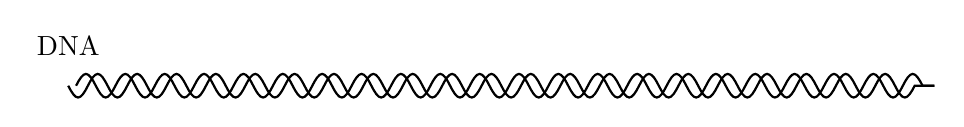
\begin{tikzpicture}[decoration={coil},
dna/.style={decorate, thick, decoration={aspect=0, segment length=0.5cm}}]
 
%DNA
\draw[dna, decoration={amplitude=.15cm}] (.1,0) -- (11,0);
\draw[dna, decoration={amplitude=-.15cm}] (0,0) -- (11,0);
\node at (0,0.5) {DNA};
 
\end{tikzpicture}
\end{document}